\subsubsection{Dense model}

This model is a forward-pass type single layer model. It has two other layers, but they do not implement logic associated with the neural network itself, but are layers of translation from matrix to vector and vice versa as explained below. Graphically, the network that has been defined is the following:

\begin{figure}[H]
    \centering
    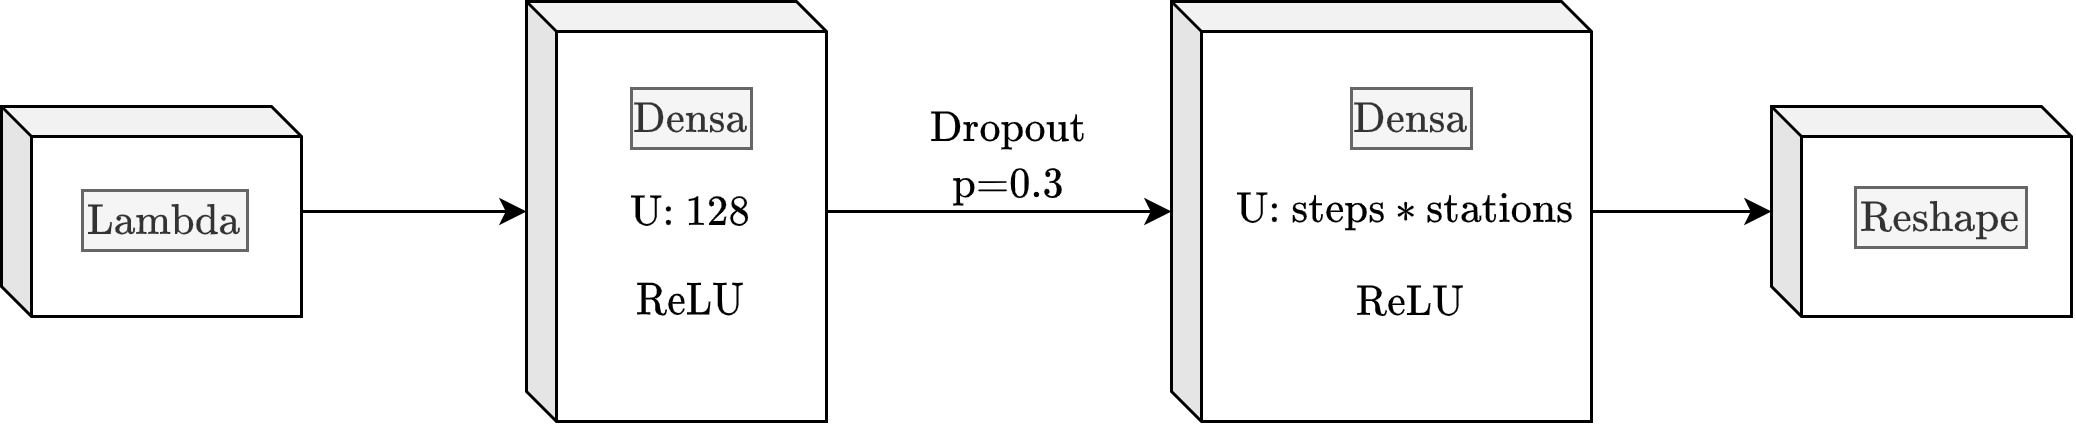
\includegraphics[width=12cm]{images/solution/models/dense.png}
    \caption{Dense model}
    \label{fig:dense-model}
\end{figure}

The first hidden layer has $128$ units. The number of layers and the number of neurons in a layer are parameters that have been set in a pseudo-random way. Different combinations have been made trying different amounts of units and 2 dense layers with $128$ units in the first one is the combination that has obtained the best results. The second hidden layer has the same amount of units that the model has to return, which is a value calculated by multiplying the number of stations with which it is working, $633$, by the number of intervals to be calculated. For example, if you want to calculate a single interval for all the stations, the vector of that layer will be $633$ elements, if you want to calculate two intervals, the number of elements of the vector will be $1266 = 2 \times 633$ and so on. This layer is common to all the models that will be explained from now on.
\newline

The last layer is a Reshape-type layer. This layer has neither an activation function nor parameters to adjust because all it does is convert the vector of the previous layer into a more understandable matrix and with which you can work more comfortably with the dataset where each row will be an interval and each column will be a station. The values of this matrix will therefore be the prediction that the model returns for the interval and station defined by its row and column in which they are found.
\newline


Following the same logic, the first layer is of the Lambda type and is in charge of performing the opposite task, given a matrix to obtain a vector. Lambda layers are layers in which the user defines a function to be executed.
\newline

The code for this model has been defined as shown below:

\begin{minted}[fontsize=\scriptsize]{python}
from tensorflow.keras.models import Sequential
from tensorflow.keras.layers import Reshape, Dense, Dropout, Lambda

# `steps` is a variable which has the number of intervals to be predict
steps = 0 

# `stations` is the number of stations in the bike network
stations = 0

dense_model = Sequential([
    # Matrix to vector
    Lambda(lambda x: x[:, -1:, :]), 
    
    # Input layer
    Dense(128, activation="relu"),

    Dropout(0.3),
    
    # Ouput layer
    Dense(steps * stations),
                  
    # Vector to matrix
    Reshape([steps, stations])
])
\end{minted}


The results of the model can be seen together with the other results in section \ref{results}.